\documentclass[titlepage]{report}
\usepackage[backend=biber,style=numeric]{biblatex}
\addbibresource{literature.bib}
\usepackage{caption}
\usepackage{subcaption}
\usepackage{graphicx}
\usepackage[utf8]{inputenc}
\usepackage[T1]{fontenc}
\usepackage{url}
\usepackage{hyphenat}
\usepackage{glossaries}
\usepackage{array}
\usepackage{calc}
\usepackage{booktabs}
\usepackage{hyperref}
\usepackage{listings}
% \usepackage{xcolor} https://tex.stackexchange.com/q/466147
\usepackage{bytefield}
\usepackage{float}
\usepackage{eurosym}
\usepackage{tabu}
\usepackage{caption}
\lstset{%
    frame=tb,
    tabsize=4,
    numbers=left,
    breaklines=true,
}
\setcounter{biburllcpenalty}{9001}
\makeglossaries{}
\newglossaryentry{ima}
{%
    name={IMA},
    description={Computer network airborne system},
    first={Integrated Modular Avionics (IMA)},
    long={Integrated Modular Avionics}
}
\newglossaryentry{dima}
{%
    name={DIMA},
    description={Distributed computer network airborne system},
    first={Distributed Integrated Modular Avionics (DIMA)},
    long={Distributed Integrated Modular Avionics}
}
\newglossaryentry{apex}
{%
    name={APEX},
    description={APplication/EXecutive Interface},
    first={APplication/EXecutive Interface (APEX)},
    long={APplication/Executive Interface}
}
\newglossaryentry{coex}
{%
    name={COEX},
    description={COre/EXecutive Interface},
    first={COre/EXecutive Interface (APEX)},
    long={COre/Executive Interface}
}
\newglossaryentry{arinc}
{%
    name={ARINC},
    description={Aeronautical Radio Incorporated},
    first={Aeronautical Radio Incorporated (ARINC)},
    long={Aeronautical Radio Incorporated}
}
\newglossaryentry{aeec}
{%
    name={AEEC},
    description={Airlines Electronic Engineering Committee},
    first={Airlines Electronic Engineering Committee (AEEC)},
    long={Airlines Electronic Engineering Committee}
}
\newglossaryentry{lru}
{%
    name={LRU},
    description={Line-Replaceable Unit},
    first={Line-Replaceable Unit (LRU)},
    long={Line-Replaceable Unit},
    plural={LRUs},
    firstplural={Line-Replacable Units (LRUs)}
}
\newglossaryentry{lrm}
{%
    name={LRM},
    description={Line-Replaceable Module},
    first={Line-Replaceable Module (LRM)},
    long={Line-Replaceable Module},
    plural={LRMs},
    firstplural={Line-Replacable Modules (LRMs)}
}
\newglossaryentry{arinc429}
{%
    name={ARINC 429},
    description={ARINC standard for a global data bus in aviation},
    first={ARINC 429 standard},
    long={ARINC 429 standard}
}
\newglossaryentry{arinc629}
{%
    name={ARINC 629},
    description={ARINC standard for a global computer bus in aviation},
    first={ARINC 629 standard},
    long={ARINC 629 standard}
}
\newglossaryentry{arinc650}
{%
    name={ARINC 650},
    description={ARINC standard for IMA packaging and interfaces},
    first={ARINC 650 standard},
    long={ARINC 650 standard}
}
\newglossaryentry{arinc651}
{%
    name={ARINC 651},
    description={ARINC report that provides guidelines for a maintenance strategy for IMA-equipped airplanes},
    first={ARINC 651 report},
    long={ARINC 651 report}
}
\newglossaryentry{arinc653}
{%
    name={ARINC 653},
    description={ARINC standard for space and time partitioning},
    first={ARINC 653 standard},
    long={ARINC 653 standard}
}
\newglossaryentry{arinc659}
{%
    name={ARINC 659},
    description={ARINC standard for a backplane data bus},
    first={ARINC 659 standard},
    long={ARINC 659 standard}
}
\newglossaryentry{RTCA}
{%
    name={RTCA},
    description={Radio Technical Commission for Aeronautics (RTCA)},
    first={Radio Technical Commission for Aeronautics (RTCA)},
    long={Radio Technical Commission for Aeronautics}
}
\newglossaryentry{do178b}
{%
    name={DO-178B},
    description={Certification for safety-critical software by the RTCA},
    first={DO-178B},
    long={DO-178B}
}
\newglossaryentry{do178c}
{%
    name={DO-178C},
    description={Certification for safety-critical software by the RTCA (replaces DO-178B)},
    first={DO-178C},
    long={DO-178C}
}
\newglossaryentry{us}
{%
    name={US},
    description={United States of America. Short: United States},
    first={United States (US)},
    long={United States}
}
\newglossaryentry{io}
{%
    name={I/O},
    description={input and output},
    first={input and output (I/O)},
    long={input and output}
}
\newglossaryentry{cpu}
{%
    name={CPU},
    description={The CPU consists of registers for fast computation and an Algorithmic Logic Unit (ALU)},
    first={Central Processing Unit (CPU)},
    long={Central Processing Unit}
}
\newglossaryentry{ram}
{%
    name={RAM},
    description={RAM is very fast memory for temporary storing data},
    first={Random Access Memory (RAM)},
    long={Random Access Memory}
}
\newglossaryentry{nist}
{%
    name={NIST},
    description={United States institute for promoting innovation and industrial competitiveness},
    first={National Institute of Standards and Technology (NIST)},
    long={National Institute of Standards and Technology}
}
\newglossaryentry{saas}
{%
    name={SaaS},
    description={},
    first={Software as a Service (SaaS)},
    long={Software as a Service}
}
\newglossaryentry{paas}
{%
    name={PaaS},
    description={},
    first={Platform as a Service (PaaS)},
    long={Platform as a Service}
}
\newglossaryentry{iaas}
{%
    name={IaaS},
    description={},
    first={Infrastructure as a Service (IaaS)},
    long={Infrastructure as a Service}
}
\newglossaryentry{hsd}
{%
    name={HSD},
    description={},
    first={Horizontal Situation Display (HSD)},
    long={Horizontal Situation Display}
}
\newglossaryentry{arp4754}
{%
    name={ARP4754},
    description={Guideline for the development of aircraft systems by SAE International},
    first={Aerospace Recommended Practic (ARP) 4754},
    long={Aerospace Recommended Practic 4754}
}
\newglossaryentry{dal}
{%
    name={DAL},
    description={Design Assurance Level},
    first={Design Assurance Level (DAL)},
    long={Design Assurance Level}
}
\newglossaryentry{idal}
{%
    name={IDAL},
    description={Item Development Assurance Level},
    first={Item Development Assurance Level (IDAL)},
    long={Item Development Assurance Level}
}



\title{From the Cloud to the Clouds: Taking Integrated Modular Avionics on a New Level with Cloud-Native Technologies}
\author{Christian Rebischke\\
Clausthal University of Technology\\
Student ID: 432108 \\
E-Mail: Christian.Rebischke@tu-clausthal.de}
\begin{document}
\maketitle
\chapter*{Acknowledgement}
\chapter*{Statutory Declaration}
This master thesis is submitted in partial fulfilment of the requirements for the Clausthal
University of Technology. I hereby declare that this dissertation is my own work and
contains nothing which is the outcome of work done in collaboration with others,
except as specified in the text and acknowledgements. The contributions of any other
supervisors to this thesis are made with specific reference.
\\
\\
Clausthal-Zellerfeld, \today
\\
\\
Christian Rebischke
\chapter*{Abstract}
The goal of this scientific work is to apply transfer knowledge from the cloud computing area to avionics and to
contribute to a more heterogeneous research picture. The focus of this work lies in particular in the transformation
of avionics architectures from a federated system to an integrated system, as well as its future development.
The challenges and solutions of known architectures will be analyzed and compared with new
achievements in cloud computing. In particular
the Service Orientated Architecture (SOA) approach plays a role in this comparison, as well as its
reliable, secure and cost-effective deployment in airplanes, drones or spaceships.
The master thesis is structured as follows: In the introduction, the classification of the thesis is repeated
and put in context with the current state of the art. Then, in the second chapter, the path from a federated
avionics architecture to an integrated system will be shown and its problems, challenges
and ideas will get isolated. This gained information is subsequently being compared with current cloud native technologies
and potential solutions for these subject will be proposed.

\chapter*{Zusammenfassung}
Ziel dieser wissenschaftlichen Arbeit ist es Transferwissen aus dem Cloud Computing Bereich auf die Avionik
anzuwenden und dazu zu einem heterogeneren Forschungsbild beizutragen. Im Fokus der Arbeit liegt insbesondere
der Weg der Avionik Architekturen von einem föderierten System hin zu einem integrierten System, sowie dessen
zukünftige Weiterentwicklung. Dabei sollen die Herausforderungen und Lösungen von bekannten Architekturen
analysiert und mit neuen Errungenschaften aus dem Cloud Computing Bereich verglichen werden. Insbesondere
der Service Orientierted Architecture (SOA) Ansatz spielt in diesem Vergleich eine Rolle, sowie dessen
zuverlässige, sichere und kostengünstige Einsatzmöglichkeiten in Flugzeugen, Drohnen oder Raumschiffen.
Die Masterarbeit ist wie folgt gegliedert: In der Einleitung wird die Einordnung der Arbeit wiederholt
und in einen Zusammenhang mit der Gegenwart gestellt. Im Zweiten Kapitel wird dann der Weg von einer föderierten
Avionik Architektur zu einem integrierten System beleuchtet und dessen Probleme, Herausforderungen
und Ideen isoliert. Diese gewonnenen Informationen werden nachfolgend aktuellen Cloud Native Technologien
gegenüber gestellt und potentielle Lösungen vorgeschlagen.

\tableofcontents
\chapter{Introduction}\label{chapter:introduction}
The number of performed flights by global airline industries increased from 23.8 million flights (2004)
to 38.9 million flights (2019)\cite{STATISTA}. This growing number of performed flights puts an enormous
pressure on the global aviation industry as a whole. The permanent price pressure lead to demands of
cheaper, lighter and smaller flight components\cite{prisaznuk1992integrated}. Every inch and every gramm 
counts in the global business of civil aviation, because every inch less means one possible paying customer 
more on the plane and every gramm less means less expensive fuel demands for the flight. But it is not only
the underlying architecture and the corresponding hardware that plays a big role in the aviation business.
The software forming these architectures and running on these devices plays an equal important role
in the aviation industry. The development of software is difficult, error-prone, tedious and expensive. This leads
to the question why the aviation industry is not exploiting resources and development processes from other industry branches.
The open source software movement provides a staggering amount of different technologies for solving problems
that are not too different to the problems from the aviation industry. Reasons for this development paralysis
are regulation and certification. The civil aviation sector is strictly regulated, thus experimenting with alternatives
is expensive and difficult. Furthermore, the existing certification companies are not known for their disruptive
technology announcements. Nevertheless this thesis tries to explore a few of these alternatives and tries to
suggest topics that might be interesting for further research. Hopefully it will help justifying further research
in this area and incite changes in the inflexible regulation and certification chain. The \gls{us} military sector 
and the \gls{us} space industry seem to be more willing to experiment with new or existing open source software. 
For example, the private \gls{us} space company \emph{SpaceX} had tremendous success with Linux as operating 
system on their \emph{Dragon} spacecraft\cite{gruen2012linux} and Linux is not only being used by 
SpaceX\cite{leppinen2017current}. Of course this success is only possible, because the space industry 
is much more isolated and kept secret than the civil aviation industry with their international standards and 
guidelines. One of these standards is the \gls{do178b} certification and its successor \gls{do178c} from the \gls{RTCA}. 
This certification has strict requirements on flight operating systems. A few of these requirements are real-time capabilities
and a transparent and documented development process with design decisions and other documents. While
real-time capabilities can be easily added via soft patches (\emph{SpaceX} is exactly doing this with their
\emph{Dragon} spacecraft\cite{gruen2012linux}), the documentation and development process seem to be an invincible
obstacle for a successful certification process. Another prominent example of open source adoption is the operation
of the Cloud Native container orchestration engine Kubernetes in military fighter planes, like the \gls{us} military
plane \emph{U-2}\cite{U2Kubernetes}. Unfortunately there is no research on that topic. This thesis tries to change this
as well and tries to connect existing research in both areas for creating synergies between them, but for connecting
these two areas we need to understand both of these areas first. 
Therefore, the next chapter will give an introduction to the history of software architectures on planes and will highlight the 
most important challenges in these.

\chapter{Related Work}\label{chapter:related_work}
\section{Federated Avionics}\label{section:federated_avionics}
To understand the background of this thesis better it is recommended to understand the journey of flight system architectures.
Around the 1970's avionics systems evolved from traditional point-to-point wiring to a standard data bus with a federated system
architecture\cite{xiong2009advanced}. This federated system
has been implemented as distributed collection of dedicated computing resources consisting of \glspl{lru} or \glspl{lrm}\cite{watkins2007transitioning}.
\glspl{lru} and \glspl{lrm} are modular components that are specifically designed for pre-determined tasks, such as
interacting with certain flight sensors/effectors\cite{lemke1985comparative}.
Sensors are reading data and effectors are executing certain actions, for example moving the flight gears.
The main advantages of \glspl{lru} are their atomic behavior and their strict and easily certifiable system design.
Each \gls{lru} or \gls{lrm} contains one specific avionic workload and its required computing resources (processors, 
\gls{io} modules, main memory, hard disks and network cards). \autoref{fig:federated_architecture} shows a simplified model
of the federated architecture with distributed \glspl{lru}, sensors, effectors, and a global data bus connecting the components.
It visualizes the enormous effort and the huge amount of cables. Duplicating the systems achieves service redundancy and ensures
system reliability\cite{prisaznuk1992integrated}, for the price of duplicating the \gls{lru} as a whole. This does not
only mean a duplicated hosted function (the actually functionality of the \gls{lru}), it also means double as much cables,
processors, main memory, network cards and connectors. Weight and complexity disadvantages are not the only problems with the federated
architecture approach. Having a dedicated hardware stack for each \gls{lru} means not fully saturated potential. Due to safety reasons
the \gls{lru} will very unlikely use all of its resources. This means there will be always a spare amount of main memory, hard disk
or network saturation. Added up over the whole federation architecture this means a huge amount of unused resource potential and unnecessary
energy consumption that could be used for other functionality. The task-specific development of \glspl{lru} leads to problems with 
functionality extensions, meaning that \glspl{lru} are not easily upgradable or extendable and therefore adjustable to new tasks or functionality.
Moreover in the past the development of federated architecture components has been closed source and very vendor specific. Specifications for
federated architecture components were mostly hidden behind a paywall or non disclosure agreements leading to a decreased developer efficiency
and less market competition due to monopolism. \glspl{lru} are not easily exchangable between vendors. \autoref{fig:federated_architecture_components}
displays the internal structure of the \gls{lru} and its interaction with other \gls{lru}. Each \gls{lru} provides its own hardware stack and hosts
exactly one avionic function. It is possible for one \gls{lru} to speak with multiple sensors or effectors, but this does not change their core
purpose of hosting exactly one function. In \autoref{section:integrated_modular_avionics} this thesis will investigate the next
step in the evolution of flight system architectures and how the disadvantages of federated architectures can be fixed.

\begin{figure}
    \centering
    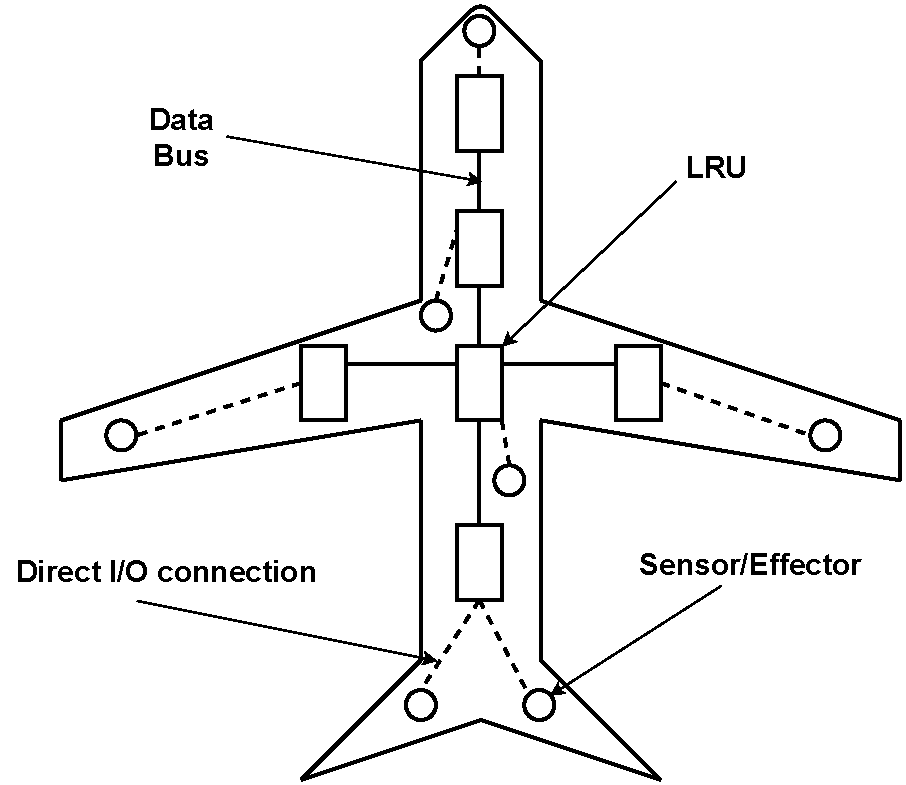
\includegraphics[width=1.0\textwidth]{figures/federated_architecture.pdf}
    \caption{Simplified visualization of the federated avionics architecture, showing \gls{lru}, sensors, effectors, and the global data bus}\label{fig:federated_architecture}
\end{figure}
\begin{figure}
    \centering
    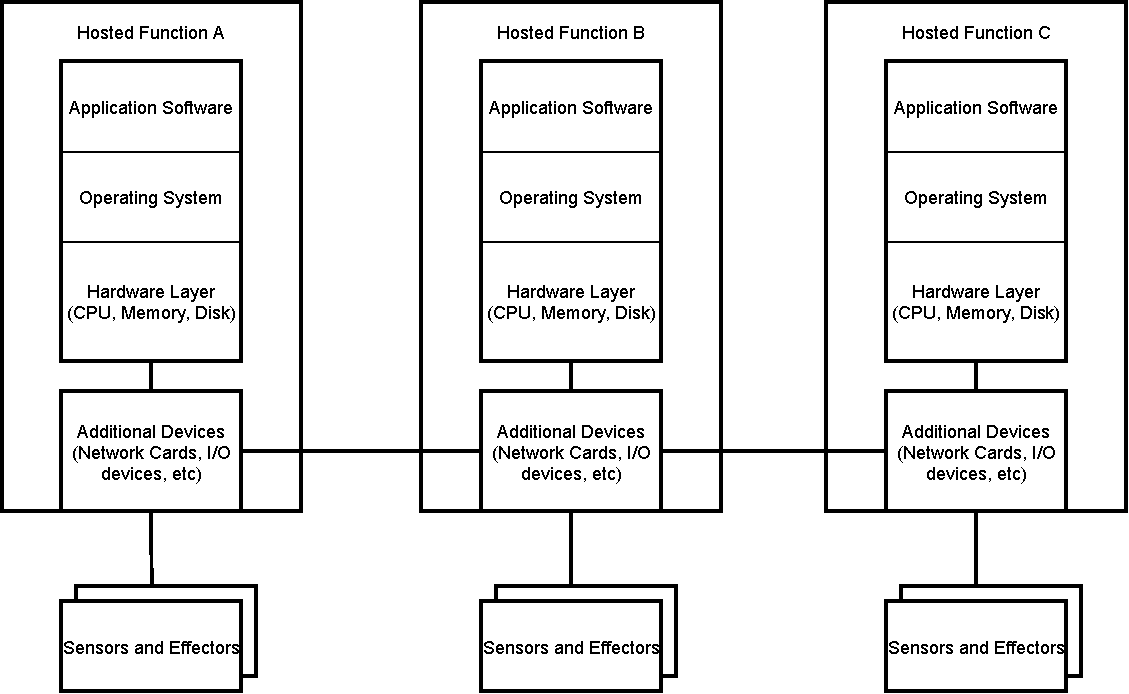
\includegraphics[width=1.0\textwidth]{figures/federated_architecture_components.pdf}
    \caption{Internal system architecture and interaction between \glspl{lru}}\label{fig:federated_architecture_components}
\end{figure}

\section{Integrated Modular Avionics}\label{section:integrated_modular_avionics}
\glsfirst{ima} is the direct successor of the federated avionics architecture. The idea behind \gls{ima}
is to consolidate the distributed hardware in flight cabinets. Flight cabinets are very similar
to racks in a datacenter. They can host multiple processing units or server blades, each comes with its own hardware stack
consisting of a \gls{cpu}, \gls{ram}, disk space and connectors for input and output\cite{prisaznuk1992integrated}. These servers are then plugged-in 
into the flight cabinet. Each server can host more than one avionic function and each function is allocated on partitions.
Partitions can be created on different ways and has been standardized in \gls{arinc653}\cite{vanderleest2010arinc}. The most common approach
is the use of a hypervisor (how this is implemented is being discussed in \autoref{section:workload_partitioning_strategies}). 
The flight cabinet provides power and required network connection to the plane's global data bus
as described in \gls{arinc629}\cite{isik2010arinc} or \gls{arinc429}\cite{fuchs2012evolution}. \gls{arinc629} is the successor of the data bus \gls{arinc429}.
Effectors and sensors communicate with the flight cabinet over \gls{arinc629}\cite{prisaznuk1992integrated}.
Sensors or effectors that are incompatible with \gls{arinc629} may communicate over remote data concentrators. Remote data concentrators are gathering data from sensors
or sending data to effectors over traditional \gls{io} connections. The gathered data or the received actions are communicated via \gls{arinc629} or \gls{arinc429}. Therefore,
remote data concentrators act as bridges between such devices and the data bus.
Using central flight cabinets cannot replace all \glspl{lru} in the plane\cite{watkins2007transitioning}. These \glspl{lru} needs to be either integrated into the flight cabinets
or connected to the global data bus, for example via remote data concentrators. \autoref{fig:ima} depicts a simplified view on integrated modular avionics architecture in a plane.
The number of \glspl{lru} has been reduced and flight cabinets has been introduced. Remote data concentrators are working as bridges between sensors and effectors incompatible
with the data bus standard and the hosted functions in the flight cabinets. \autoref{fig:ima_components} shows the modules inside of such a flight cabinet. The flight cabinet
possesses multiple processing units. Each processing unit is comparable to a dedicated computer with its own hardware and operating system. These processing units
are being connected via a network layer and each processing unit hosts one or more hosted functions. Hosted functions are isolated from each other and have
a fixed predetermined set of resources and execution time.

\begin{figure}
    \centering
    \includegraphics[width=1.0\textwidth]{figures/ima.pdf}
    \caption{Simplified visualization of the integrated modular avionics architecture, showing sensors, effectors, cabinets and the data bus \glspl{lru}}\label{fig:ima}
\end{figure}

\begin{figure}
    \centering
    \includegraphics[width=1.0\textwidth]{figures/ima_components.pdf}
    \caption{View into a flight cabinet}\label{fig:ima_components}
\end{figure}


Another important factor of avionic functions hosted in flight cabinets is that they differ in reliability requirements. For example
the system that controls the flight entertainment system is less important than the system that controls the cabin air supply or the temperature. 
Hence, every hosted function needs a priority level.


\section{Distributed Integrated Modular Avionics}\label{section:distributed_integrated_modular_avionics}

\section{Workload Partitioning Strategies}\label{section:workload_partitioning_strategies}
\nocite{*}
\printbibliography{}
\lstlistoflistings{}
\listoftables{}
\listoffigures
\glsaddallunused
\printglossary{}
\end{document}
